\section{代数闭域上的约态概形}

概形概念的发始,即是想要推广经典的代数闭域上的仿射簇,我们将从它开始一系列关于概形的例子。在这里,代数闭域$K$上的仿射簇是指一个仿射概形$\spec R$,其中$R$是一个簇$X$的坐标环\index{坐标环},即$R$是一个有限生成的约态$K$\hyp 代数\index{约态!代数}。(回忆一个环是约态的,是指它没有非零幂零元。)$\spec R$时常被叫做\textit{相伴于簇}$X$的概形\footnote{译者注:在下面的行文中,翻译中也会将$\spec R$称为$X$的相伴概形。同时,有时候也会反过来,称一个簇或者闭点相伴于某个概形。由于有时候一个理想也给出一个簇,所以有时也会用相伴于理想的概形,或者理想的相伴概形等说法。}:这种概形有时就直接被称作仿射簇。在以后几节中,我们将考虑不同于这个基本模型的概形。

相伴于代数闭域$K$上的仿射簇的$K$\hyp 概形与这个簇是等价的对象:它们都可以决定一个相同的坐标环或者被一个相同的坐标环决定。但是,在这个例子中已经有所表现的是,一些经典的概念,比如簇的相交或者映射的纤维,在概形理论中会有更精确的意思。我们将在这节以及接下来的章节中看到这个现象的例子。

\subsection{仿射空间}

我们从概形$\mathbb{A}^n_K:=\spec K[x_1$, $\dots$, $x_n]$开始,其中$K$是一个代数闭域。这个概形被称为$K$上的\textit{仿射}$n$-\textit{空间}。

这里将使用一个标准的但绝不平凡的代数结论 ------ Hilbert's Nullstellensatz(零点定理)的一种形式;比如可见Eisenbud [1995].

\begin{thm}[Nullstellensatz]
	设$K$是一个域,如果$\mathfrak{m}$是多项式环$K[x_1$, $\dots$, $x_n]$的一个极大理想(或者更一般地,$p$是$K$上的一个代数空间的子簇的一个闭点),则
	\[
		K[\text{$x_1$, $\dots$, $x_n$}]/\mathfrak{m}=\kappa(p)
	\]
	是一个有限维$K$\hyp 矢量空间。
\end{thm}

在我们的例子中,$K$是代数闭的,这就意味着$\kappa(p)=K$. 因此,记$\lambda_i$是$x_i$在$\kappa(p)$中的像,可以看到
\[
	\mathfrak{m}=(\text{$x_1-\lambda_1$, $\dots$, $x_n-\lambda_n$}).
\]
于是,$\mathbb{A}^n_K$中的闭点与$K$中元素的$n$元组相对应,正如期望的那般。有时,我们会用“点$(\lambda_1$, $\dots$, $\lambda_n)$”来指代“点$[(x_1-\lambda_1$, $\dots$, $x_n-\lambda_n)]$”. 

从一维的情况开始,仿射直线
\[
	\mathbb{A}^1_K=\spec K[x]
\]
长得就像它的经典对应,同样被叫做仿射直线的仿射簇。仿射直线上对每一个$\lambda\in K$都有一个闭点,闭点构成的集合上的Zariski拓扑也与仿射簇上的经典的Zariski拓扑相同:开集是有限集的补。概形$\mathbb{A}^1_K$与簇不同的地方只在于它多了一个点,这个点被称为\textit{一般点}\index{一般!点}\footnote{译者注:作者没给出明确的定义,这里给一下:如果$Y=\overline{\{x\}}$,则称$x$是$Y$的一个一般点。一般而言,一般点可能不存在,也可能不唯一的。},对应于零理想$(0)$。
\vspace{-1ex}\begin{center}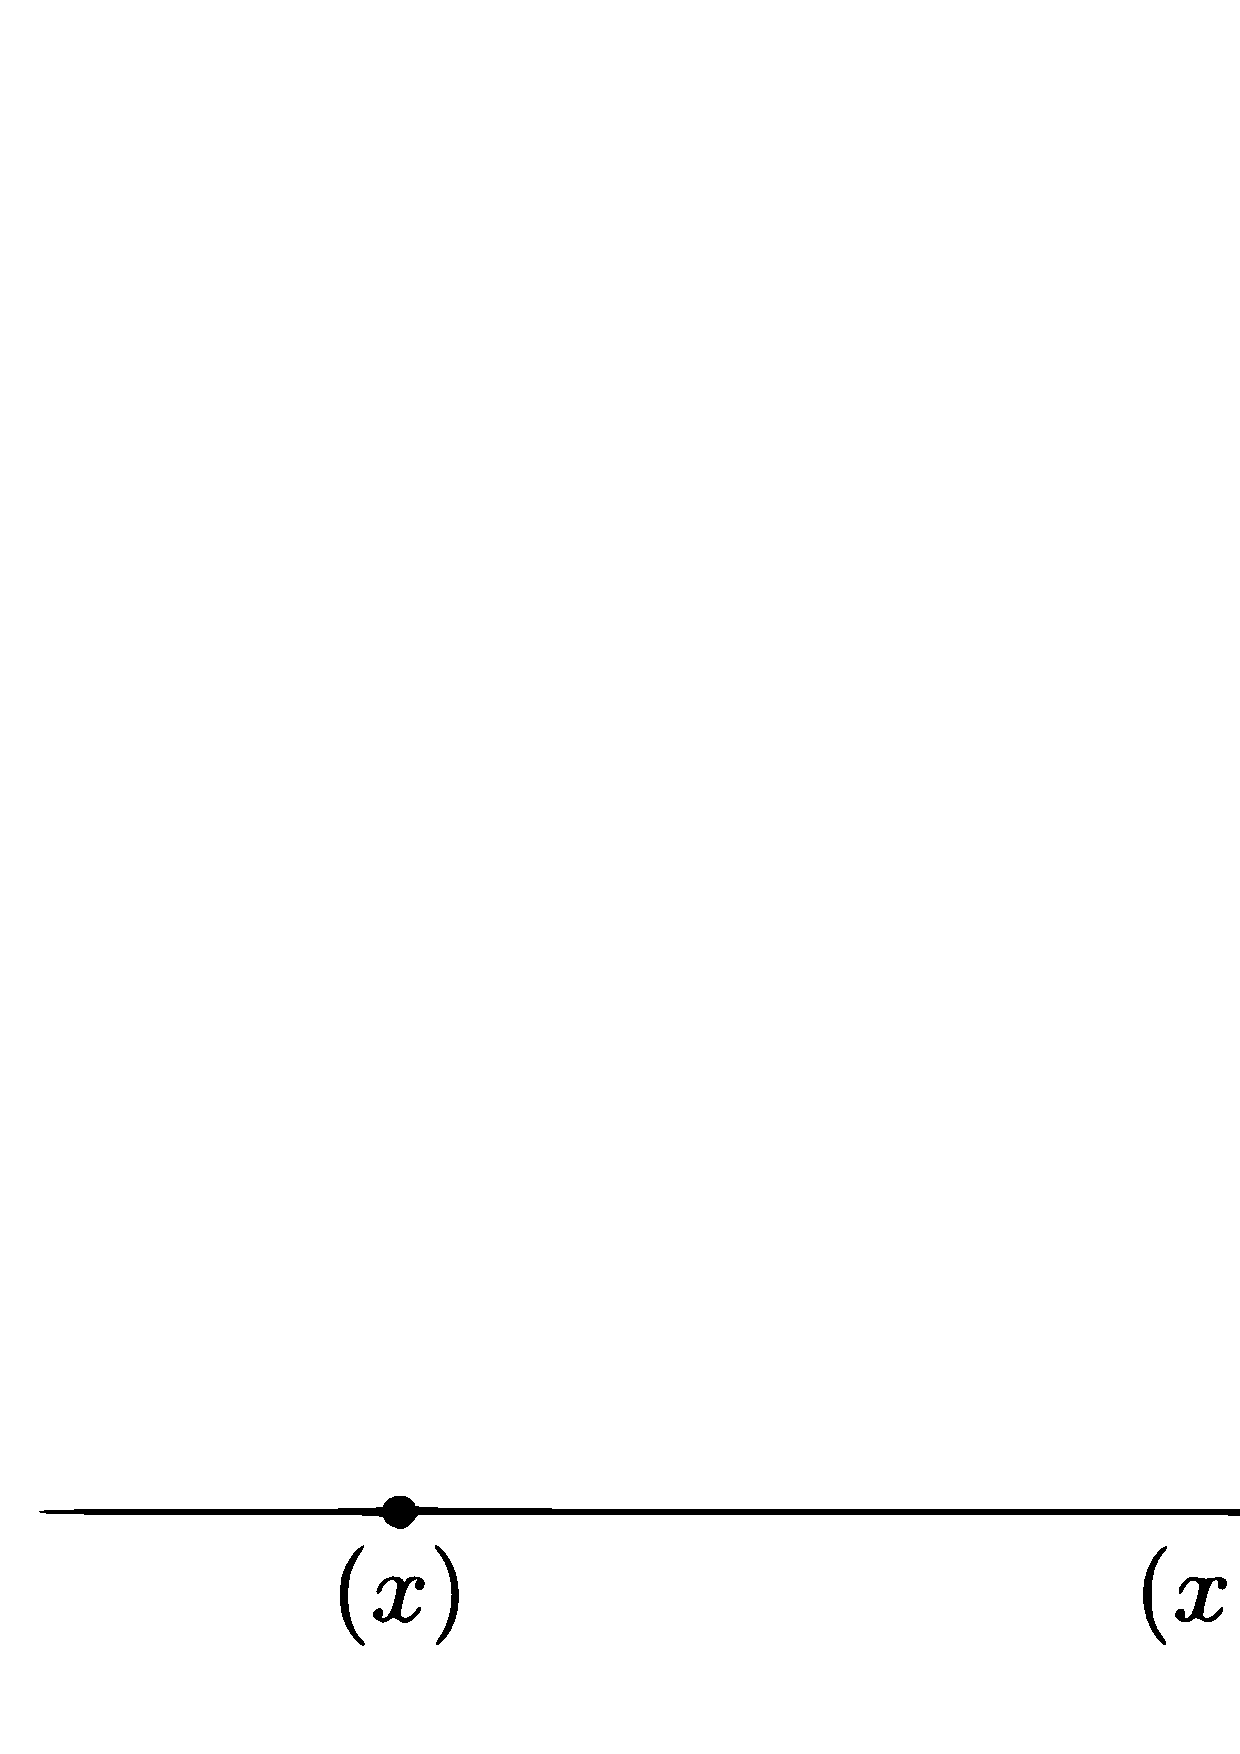
\includegraphics[scale=\scale,bb=0 0 447 81]{\PICDIR/1.png}\end{center}
\vspace{-2ex}点$(0)$的闭包是整个$\mathbb{A}^1_K$,因此,$\mathbb{A}^1_K$的闭子集就是$\mathbb{A}^1_K-\{(0)\}$的有限子集。

仿射平面$\mathbb{A}^2_K=\spec K[x,y]$同样与它的经典对应相似,但现在就多了许多点,同时也表现得更加有趣。像之前一样,我们有来自于极大理想$(x-\lambda,y-\mu)$的闭点,对应于寻常平面中的$(\lambda,\mu)$. 但现在却有两类非闭点。首先,对每一个不可约多项式$f(x,y)\in K[x,y]$,有一点$p$对应于素理想$(f)\subset K[x,y]$,它的闭包包含$p$本身以及所有使得$f(\lambda,\mu)=0$的闭点$(\lambda,\mu)$,点$(f)$被称为该集合的一般点。一般地,概形中的每一个点都被称为该点闭包的一般点。比起簇$\mathbb{A}^2_K$,概形$\mathbb{A}^2_K$中我们需要对每一条不可约平面曲线加入一点,这个新的点属于这条曲线的闭包,并且该点的闭包等于曲线的闭包。最后,正如在$\mathbb{A}^1_K$中,我们还需要加入一个对应于零理想的点,即$\mathbb{A}^2_K$的一般点,它的闭包是整个$\mathbb{A}^2_K$.

\begin{center}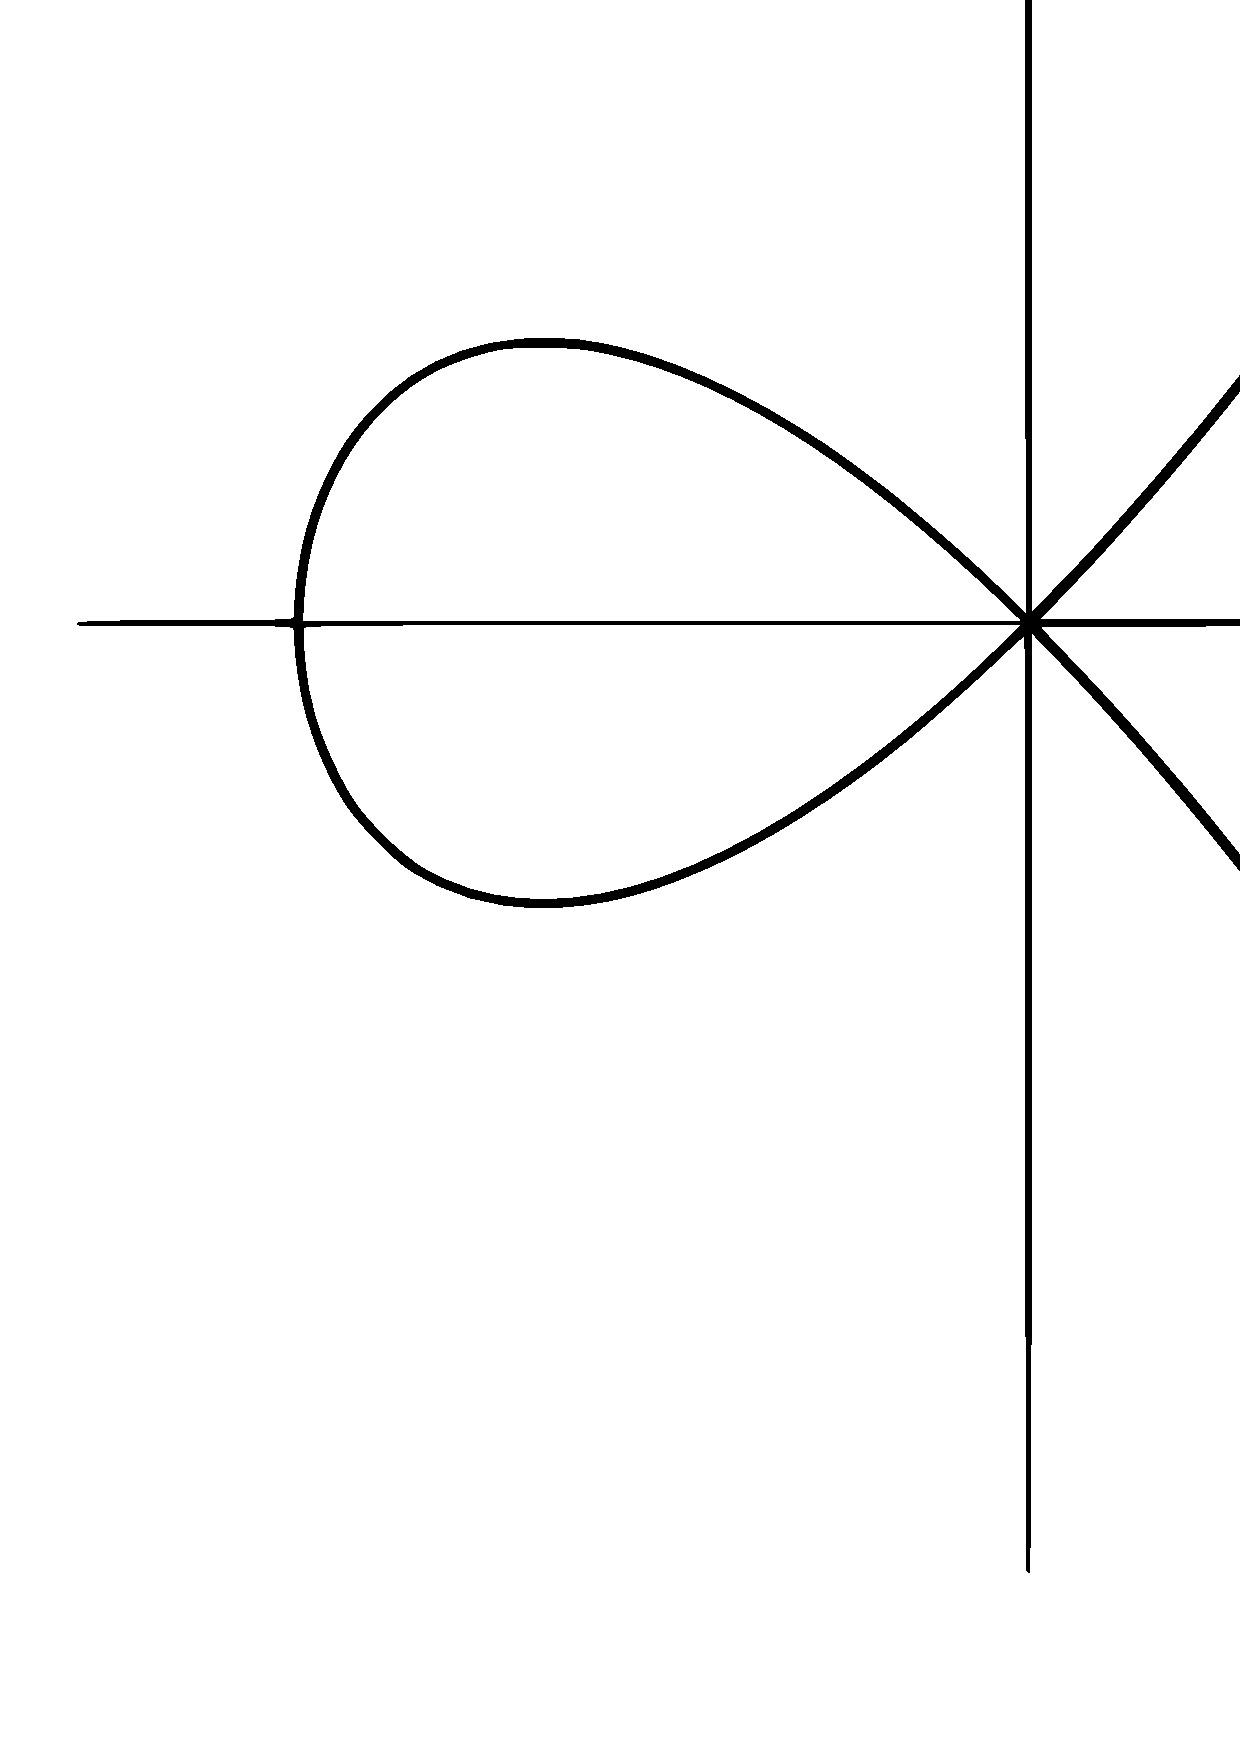
\includegraphics[scale=\scale,bb=0 0 688 413]{\PICDIR/2.png}\end{center}

因为$K[x,y]=K[x]\otimes_K K[y]$,从定义有
\[
	\mathbb{A}^2_K=\mathbb{A}^1_K\times_{\spec K}\mathbb{A}^1_K.
\]
在这里,纤维积显然是一个正确的积,但它作为集合并不等于其因子作为集合的积。

仿射空间$\mathbb{A}^n_K$的情况是上一个例子的直接推广:几何上,可以看到概形$\mathbb{A}^n_K$是经典的仿射$n$-空间对每一个正维数的不可约子簇$\Sigma$加上一点$p_\Sigma$. 与前面一样,$p_\Sigma$属于$\Sigma$的闭包中,且$p_\Sigma$的闭包等于$\Sigma$的闭包,是$\Sigma$的一般点。

更一般的,设$X\subset \mathbb{A}^n_K$是任意的仿射簇,对应于理想$I\subset \mathbb{A}^n_K$以及坐标环$R=K[x_1$, $\dots$, $x_n]/I$,我们能得到相伴的仿射概形$\spec R$,并可以通过商映射$K[x_1$, $\dots$, $x_n]\to R$将它看作$\mathbb{A}^n_K$的一个子概形。这个概形,与$\mathbb{A}^n_K$的情形类似,长得就像仿射簇$X$但还需要对每一个正维数的不可约子簇$\Sigma\subset X$加入一个新的一般点$p_\Sigma$.

纤维,或者更一般的原像,是除了簇之外,概形最有可能出现在经典代数几何中的方式。

\begin{exe} \label{exe.2.2}
设$\varphi:K[x]\to K[x]$是一个环同态,他将$x$变成$x^2$,考虑$\varphi$诱导的$\spec K[x]$到自身的映射。证明,在概形意义上,点$0$的纤维是由$(x^2)$定义的子概形。

\begin{center}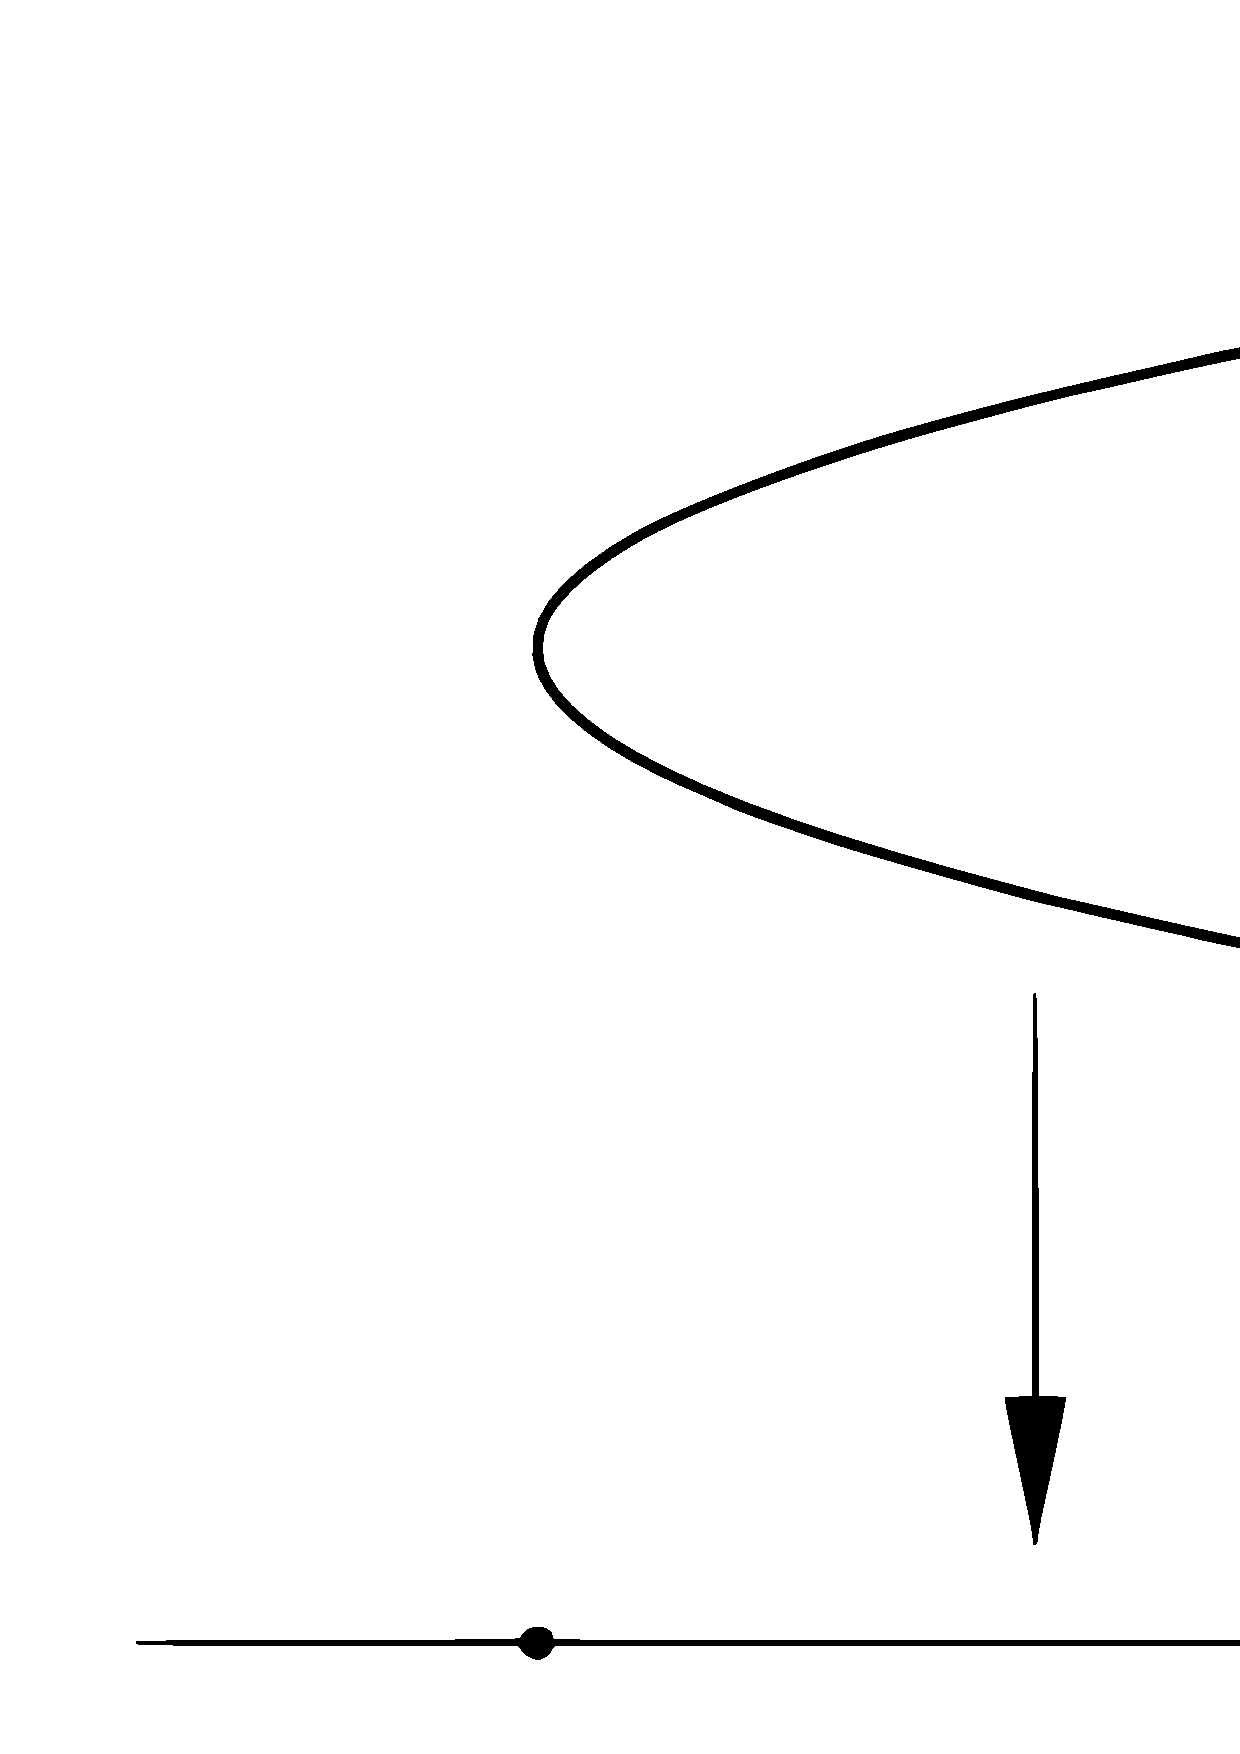
\includegraphics[scale=\scale,bb=0 0 507 309]{\PICDIR/3.png}\end{center}
\end{exe}

在所有的概形中,代数闭域上仿射簇的相伴概形被如下性质的环$R$的谱所刻划,
\begin{compactitem}[~~~--]
\item 有限生成
\item 约态代数\index{约态!代数}
\item 在一个域上
\item 这个域是代数闭域
\end{compactitem}

为了对更一般的概形长成哪样有所感觉,以及对它们有什么益处有所把握,我们在接下来的几节中考虑当撤去上面的几条四条限制后将会发生什么。我们会主要考虑那些上面四条限制中只有一条不满足的情况,因为理解它们将使得我们可以理解更一般的情况;偶尔会在习题中提到更复杂的例子。

\subsection{局部概形}

我们的第一类不同于簇的概形的例子是局部环的谱,称之为\textit{局部概形}\index{局部!概形}。我们这里将考虑的例子是代数闭域上的约态代数的谱,但不一定是有限生成的。局部概形常常作为技术性工具来研究其他更几何的概形:它们经常被用来将注意力集中在一个仿射概形的局部结构上。在只有一个闭点的例子中,概形比起簇新增的点将变得更加醒目。自然,只用一个几何点来表示这些概形是错误的,取而代之的,它们应当被看成簇的芽。只有一个闭点的现象不是新近才被代数学家研究的,作为类似物,当考虑复解析流形上一点处的芽时它已经出现了,那里它给出了一点$x$处“足够小”的邻域的图像:比如,在这个“足够小”的邻域中,每条经过$x$的曲线都可以被区分开来,尽管它们可能除了$x$之外再无在任意的邻域中有定义的点。我们将在局部环的谱上看到类似的图像。

首先考虑环$K[x]$关于极大理想$(x)$的局部化$K[x]_{(x)}$,令$X=\spec K[x]_{(x)}$. 空间$|X|$只有两个点:一个闭点对应于极大理想$(x)$,另一个开点对应于零理想$(0)$,他的闭包包含点$(x)$. 含入同态$K[x]\hookrightarrow K[x]_{(x)}$诱导了一个映射$X\to \mathbb{A}_K^1$,于是我们将$X$看作$\mathbb{A}_K^1$的子概形(尽管$|X|$在$\mathbb{A}_K^1$不是开的也不是闭的)。子概形$X$是“局部的”,因为$X$是所有$\mathbb{A}_K^1$中包含$(x)$的开集的交\footnote{译者注:若一个拓扑空间存在一般点,则其任意开子集都包含所有的一般点。设$\mathbb{A}_K^1$中所有包含$(x)$的开集的交为$U$,因此$X=\{(0),(x)\}\subset U$. 反过来,对任意闭点$p\in \mathbb{A}_K^1$,则$\mathbb{A}_K^1-p$是一个包含$(x)$的开集,但是并不包含$p$,所以$p\not\in U$. 于是$X=U$. 这个命题可以如下推广:设$X$是一个拓扑空间,对$x\in X$,记所有$x$的开邻域的交为$S_x$,则$S_x=\{y\,:\, x\in \overline{\{y\}}\}$.},于是,比如,$X$上的正则函数正好就是$\mathbb{A}_K^1$上在点$0=(x)$处正则的有理函数,即它们是$\mathscr{O}_{\mathbb{A}_K^1}(U)$中的元素,其中$U$是$\mathbb{A}_K^1$中包含点$0=(x)$的某个邻域。在这层意味上,$X$是$\mathbb{A}_K^1$在原点处的芽。

接着,考虑概形$X=\spec R$,其中$R=K[x,y]_{(x,y)}$是$K[x,y]$关于极大理想$(x,y)$的局部化,极大理想$(x,y)$对应于点$(0,0)$. 同上,我们有映射$X\to \mathbb{A}_K^2$,这里我们能将$X$看成$\mathbb{A}_K^2$中所有$(0,0)$的邻域的交。类似地,$X$只有一个闭点,但现在却有了无穷多的非闭点,每一个都对应于一条经过原点的不可约曲线。于是,$X$的子概形是$\mathbb{A}_K^2$的子概形在$(0,0)$的芽,以及$X$本身是$\mathbb{A}_K^2$在$(0,0)$的芽。

对$\mathbb{A}_K^n$乃至对$\mathbb{A}_K^n$的每一个子概形,都有类似的构造:如果$X=\spec K[x_1,$ $\dots$, $x_n]/I\subset \mathbb{A}_K^n$一个理想为$I$的仿射簇的相伴概形,而$\mathfrak{m}$相伴于$X$的一个闭点,我们能将概形$\spec K[x_1,$ $\dots$, $x_n]_\mathfrak{m}/I_{\mathfrak{m}}$看成$X$中$[\mathfrak{m}]$的一个邻域的芽。与在许多语境中谈论一个空间上一点处的函数芽不同,在概形理论中,芽依然是一个概形。

在某些场合,这样引入的局部概形实际上还不够局部:概形处一点的局部环依然包含着许多概形整体结构的信息。比如,非奇异簇$X$的概形在不同闭点处的芽不一定是同构的,尽管当我们考虑由同一个方程定义的复解析簇$X^{\text{an}}$时,任意两点的芽确实是同构的。出现这个现象的实质在于这里用来定义芽的开集太大了。为了在概形语境下得到一个更局部的图像,我们需要观察幂级数环对应的概形:比如,比起考察$\mathbb{A}_K^2$处原点$(0,0)$某个邻域的芽$X=\spec K[x,y]_{(x,y)}$,我们转而考虑概形$Y=\spec K [\![x,y]\!]$. 与前面的例子类似,它只有一个闭点$[(x,y)]$以及一个一般点$[(0)]$,一般点的闭包是整个$Y$,此外,对每一个$x$和$y$的不可约幂级数$\sum a_{i,j}x^iy^j$,$Y$上都对应着有一点。映射
\[
	K[x,y]\hookrightarrow K[x,y]_{(x,y)}\hookrightarrow K[\![x,y]\!]
\]
给出了映射$Y\to X\to \mathbb{A}_K^2$,于是我们能把$Y$想象成比$X$“更小的”原点的邻域。(然而,注意到$X$和$Y$都不是$\mathbb{A}_K^2$的开子概形或闭子概形。)比如,如果$X$中对应于素理想$(y^2-x^3-x^2)$的曲线是不可约,且域$K$的特征不是$2$,则$\mathbb{A}_K^2$中被这个方程定义的曲线在$Y$中的原像是两个(非平凡)曲线的并。因为$x^2+x^3$有着幂级数表示的平方根
\[
	u=x+\frac{1}{2}x^2-\frac{1}{8}x^3+\cdots.
\]
因此我们能把$y^2-x^3-x^2$分解为
\[
	y^2-x^3-x^2=(y-u)(y+u),
\]
所以概形$\spec  K[\![x,y]\!]/(y^2-x^3-x^2)$是可约的。(见下图。)

\begin{center}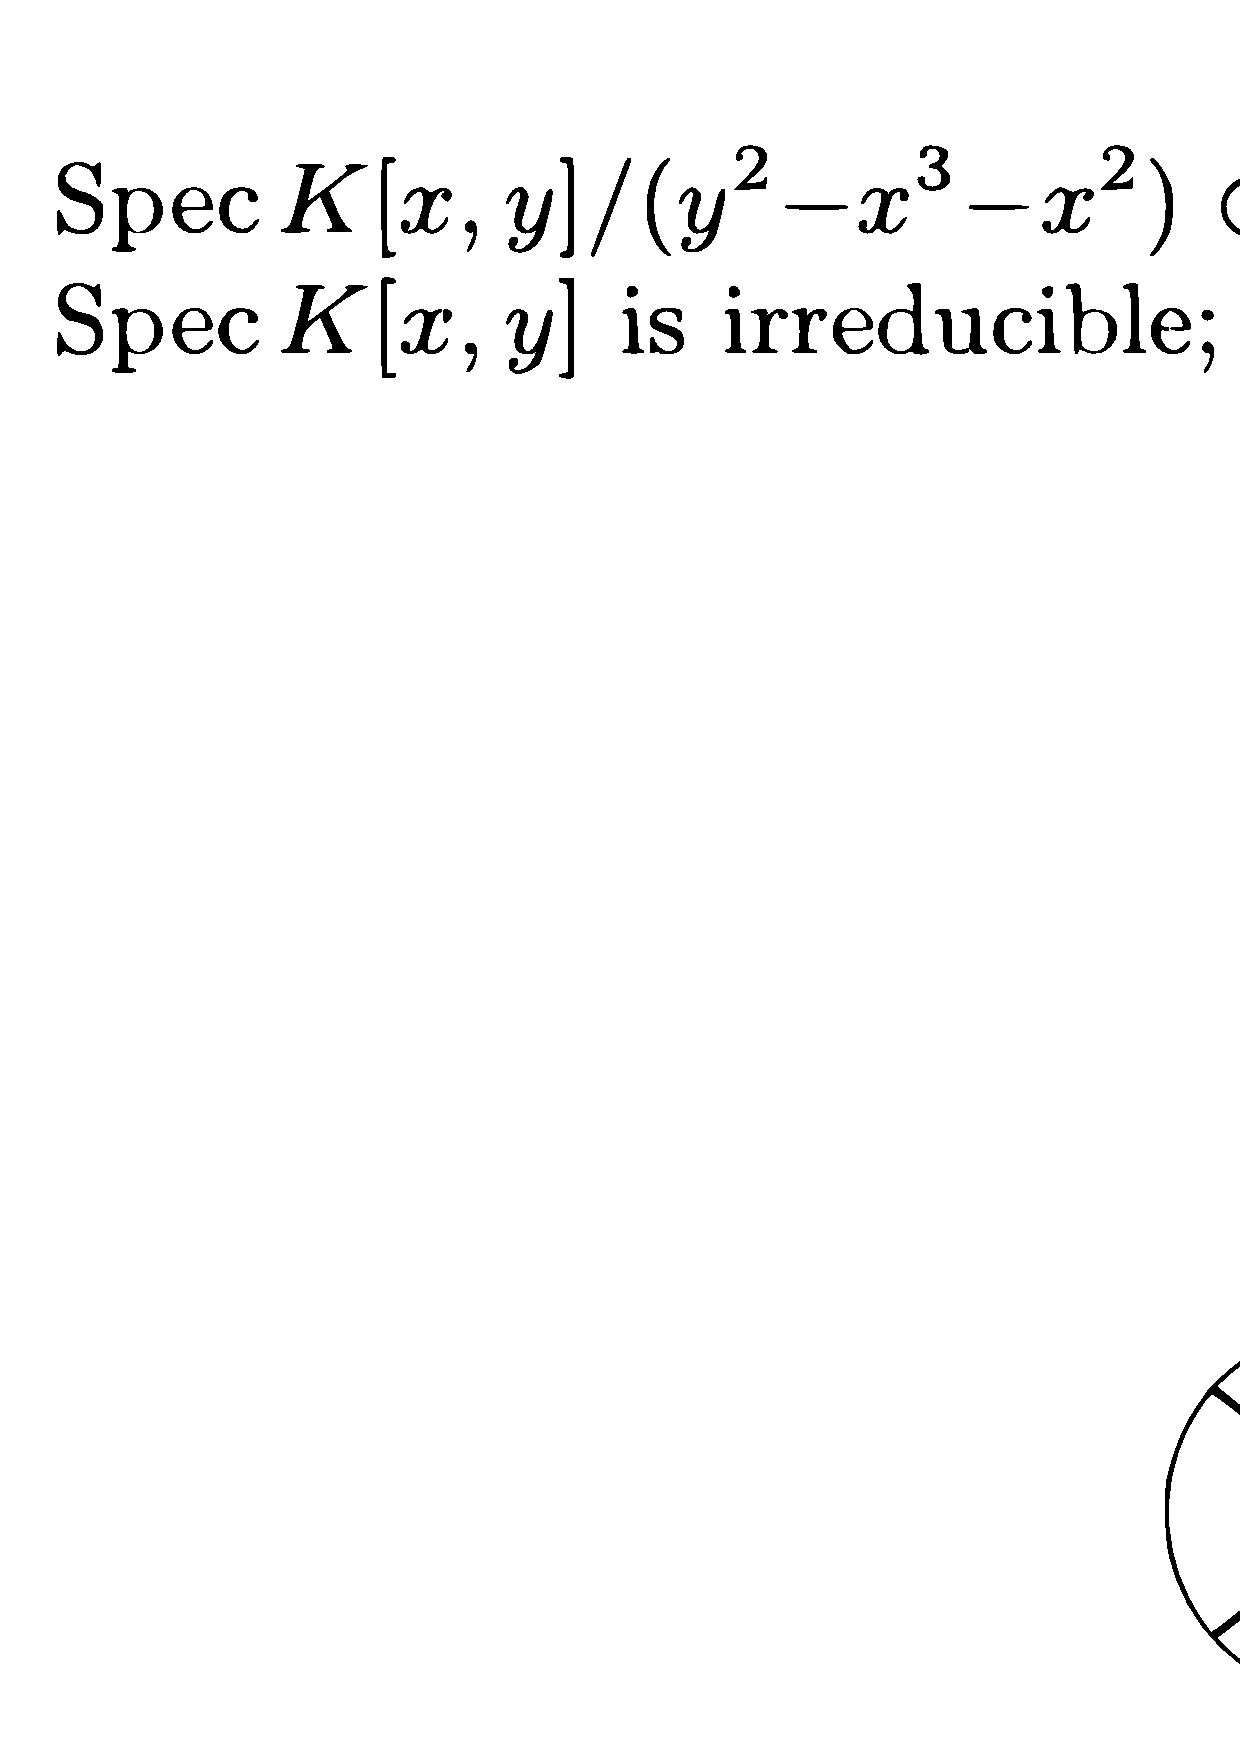
\includegraphics[scale=\scale,bb=0 0 600 444]{\PICDIR/4.png}\end{center}

当然,为使这样的事是可行的,$Y$必然比$X$有“更多”曲线,下面的习题补充了这点。

\begin{exe}
	\begin{compactenum}[(a)]
		\item 同上,设$u=\sqrt{x^2+x^3}$,那么$[(y-u)]$在$\spec K[x,y]$中的像是什么?(提示:这是一个包含$y^2-x^3-x^2$的素理想。)
		\item 证明,$Y$中的点$(y-\sum_{n\geq 1}x^n/n!)$在$\mathbb{A}_K^2$中的像是$\mathbb{A}_K^2$的一般点。
	\end{compactenum}
\end{exe}

一般地,在上面的映射$Y\to X$下,一点的原像对应于一条$\mathbb{A}_K^2$的不可约曲线$C$,它由原点处$C$的所有解析分支构成。(更多关于分支的讨论见Walker [1950]或者Brieskorn以及Kn\"{o}rrer [1986].)

虽然这里有了局部概形的另一个重要例子,但上面的概形$Y$的一个问题是,Exercise {\theexe}(b)中的点与代数的观点相去甚远。为了避免这点,我们可以转而考虑幂级数环的子环$H\subset K[\![x,y]\!]$的谱$Z$,其中环$H$在$K[x,y]$的分式域$K(x,y)$上满足一个代数方程。我们称其为概形$X$的\idx{Hensel化},概形$Z$居于$Y$与$X$之间,使得我们有一列映射
\[
	Y\to Z\to X\to \mathbb{A}_K^2.
\]
这种构造的用处在于,$H$是一系列有限生成$K$\hyp 代数的并,于是$Z$是一族概形的逆极限,这族概形每一个都来自于寻常的簇。几何上来看,$Z$是在$\mathbb{A}_K^2$在\textit{\'{e}tale拓扑}\index{\'{e}tale!拓扑}下的芽。这个概念我们这里按下不表,详细可见Artin [1971].

\begin{exe}
	当$K=\mathbb{C}$,如何将收敛幂级数构成的环的谱纳入这种图像中?
\end{exe}